\title{Star Formation and Feedback in Stellar Clusters and Galaxies.\\
       Code performance and scaling.}

\documentclass[11pt]{article}

\usepackage[letterpaper, margin=1in]{geometry}
\usepackage{amsmath}
\usepackage{natbib}
\usepackage{graphicx}
\usepackage{epstopdf}
\usepackage{titling}

\setlength{\droptitle}{-7em}   % This is your set screw
\epstopdfsetup{update}
\citestyle{aa}

\renewcommand{\floatpagefraction}{.8}%

\newcommand {\apj}{ApJ}
\newcommand {\aj}{AJ}
\newcommand {\apjs}{ApJS}
\newcommand {\apjl}{ApJL}
\newcommand {\mnras}{MNRAS}
\newcommand {\aap}{A\&A}
\newcommand {\aapr}{A\&ARv}
\newcommand {\araa}{ARA\&A}
\newcommand {\pasj}{PASJ}
\newcommand {\pasp}{PASP}
\newcommand {\bain}{Bulletin of the Astronomical Institutes of the Netherlands}
\newcommand {\fcp}{Fundamentals of Cosmic Physics}
\newcommand {\nat}{Nature}
\newcommand {\na}{New Astronomy}
\newcommand{\eg}{e.g.,}
\newcommand\rmxaa{Rev. Mex. Astron. Astrofis.} % Revista Mexicana de Astronomia y Astrofisica

\date{\vspace{-10ex}}

\begin{document}
\maketitle

\section{Introduction}
{\bf general introduction goes here... pending Josh's side}


\section{\texttt{Enzo}}

We determine the performance and scaling properties of \texttt{Enzo} in the context of the typical computational loads of our intended isolated dwarf galaxy simulations. In this situation, we are concerned with the weak scaling properties and efficiencies of \texttt{Enzo}. This analysis makes use of case studies of our dwarf galaxy model run at 1.0 and 2.0 pc resolution (note, our inteded resolution is 1.5 pc), as well as a full-physics 8 pc resolution run. The high resolution tests ran on 128 processors (64 for the low resolution case) on the TACC Stampede cluster, our proposed allocation resource.

\subsection{Computational Methodology and Algorithms}

\texttt{Enzo} is a parallel, cosmological, AMR hydrodynamics + N-body code that has been well tested and used in a variety of applications, as discussed in more detail in the main document. Below, we outline the code methodology for each piece of \texttt{Enzo} relevant to this present work; see \cite{Enzo2014} for a more detailed description of all methods. 

\subsubsection{Hydrodynamics and Gravity}

\texttt{Enzo} is equipped with multiple, distinct hydrodynamics solvers. For this work we employ a direct-Eulerian piecewise parabolic method \citep{ColellaWoodward1984, Bryan1995}. This is an explicit, higher-order accurate version of Godunov's method for ideal gas hydrodynamics that uses spatially third-order accurate piecewise parabolic monotonic interpolation. This base method is extended to multiple dimensions using directional splitting, resulting in a final algorithm that is second-order accurate in space and time; we explicitly conserve mass, linear momentum, and energy. We default to using the two-shock approximate Riemann solver, with progressive fallback to more diffusive approximate Riemann solvers when higher order methods produce negative densities or energies. The hydrodynamics time step is set by the Courant-Friedrichs-Levy (CFL) condition for stability, scaling linearly with cell size ($\Delta x$) and inversely proportional to the sum of the bulk velocity and sound speed in each cell in a given direction. 

%\texttt{Enzo} is equipped with multiple, distinct hydrodynamics solvers. For this work we employ a direct-Eulerian piecewise parabolic method \citep{ColellaWoodward1984, Bryan1995}. This is an explicit, higher-order accurate version of Godunov's method for ideal gas hydrodynamics that uses spatially third-order accurate piecewise parabolic monotonic interpolation. Shock capturing is handled with a nonlinear Riemann solver. This base method is extended to multiple dimensions using directional splitting, resulting in a final algorithm that is second-order accurate in space and time; we explicitly conserve mass, linear momentum, and energy \citep{Hawley1984, NormanWinkler1986}. We use a dual energy formalism to track the total energy and thermal energy separately, preventing substantial numerical errors that arise when the thermal energy is very small compared to the total energy (i.e. when the kinetic energy is large). We default to using the two-shock approximate Riemann solver \citep{Toro1997}, with progressive fallback to more diffusive approximate Riemann solvers when higher order methods produce negative densities or energies \citep{LemasterStone2009}. In this situation, we fall back to either the Harten-Lax-van Leer (HLL) \citep{Toro1997} method with contact discontinuities -- a three-wave, four-state solver -- or the basic HLL -- a two-state, three-wave solver. The hydrodynamics time step is set by the Courant-Friedrichs-Levy (CFL) condition for stability, scaling linearly with cell size ($\Delta x$) and inversely proportional to the sum of the bulk velocity and sound speed in each cell in a given direction. The multidimensional CFL limited time step is the harmonic average of the limiting CFL time step in each dimension. 

%Gas self-gravity and the gravitational forces of the massive star particles are computed together to compute the gravitational acceleration on each cell and particle. On the root grid, we use a cloud-in-cell (CIC) method \citep{HockneyEastwood1988} to map particles to a time-centered density field, including the effects of particles across sub-grids and neighboring domains; a similar time-centered density field is computed for the baryons in each grid cell. The gravitational potential is solved for using a fast Fourier transform (FFT) in isolated boundary conditions \citep{James1977}; accelerations are computed with a two-point centered difference scheme using the transformed real-space potential. For accuracy on sub-grids, we employ the seven-point, second-order finite difference approximation to Poisson's equation, solving the given Dirichlet boundary conditions with multigrid relaxation. Unwanted oscillations and errors across grids are reduced using expanded buffer zones around each grid, coupled with an iterative relaxation process between sibling grids. Particle accelerations are computed from the grid potential using linear CIC mapping. \texttt{Enzo} employs the particle-mesh N-body method from \cite{HockneyEastwood1988} to evolve the colissionless star particles with an effective force resolution of approximately 2$\Delta x$.

\texttt{Enzo} constructs the gravitational potential from both the gas and star particles to compute the resulting accelerations for each cell and particle. Particles are mapped to a time-centered density field using a cloud-in-cell (CIC) method \citep{HockneyEastwood1988}; this is summed together with a time-centered baryon density. The potential is solved on the root grid using a fast Fourier transform with isolated boundary conditions \citep{James1977}. For accuracy on sub-grids, we solve an approximate Poisson's equation with a second-order finite difference method and multigrid relaxation. Baryon accelerations are computed using a two-point centered difference scheme; accelerations are mapped to particles using linear CIC interpolation. \texttt{Enzo} employs a particle-mesh N-body to evolve the colissionless star particles with an effective force resolution of $\sim 2 \Delta x$.

\subsubsection{Grid Hierarchy and Parallelization Strategy}

%\texttt{Enzo} AMR simulations begin with a defined rectilinear root grid encompassing the computational domain. Additional levels of refinement take the form of child sub-grids nested within the root grid, generating a nested tree comprised of grid parents, children, and siblings; for our purposes, additional sub-grids increase resolution by a factor of two. Each grid is comprised of active zones and ghost zones that store boundary information from sibling grids. Each level in this tree is evolved on independent time steps, reducing unneeded computation on lower levels of refinement.

\texttt{Enzo} AMR simulations begin with a rectilinear root grid encompassing the computational domain. Additional levels of refinement take the form of child sub-grids, nested within the root grid; the grid hierarchy then consists of parent, child, and sibling grids. Grids contain both active and boundary (ghost) zones used for sharing sibling grid information. Each level in the grid hierarchy is evolved on independent time steps, reducing unneeded computation. 
%Using grid objects as fundamental units that exist entirely on a single processor, \texttt{Enzo} has been parallelized with the message passing interface (MPI). Grids are therefore distributed among processors in such a way to attempt to balance the computational load across processors. This is simple for the root grid, which is evenly divided in tiles to all processors, but is more complicated for higher refinement levels, which usually are not uniformly distributed in the simulation volume. Higher levels of refinement are initially placed on the processors that host their parent grids, but are subsequently distributed among other processors to reduce computational load. Load is estimated as the number of active zones on each grid. We use a simple load-balancing option to progressively move grids from processors with high computational loads to processors with the lowest computational loads until the load ratio of the most-to-least loaded processors is less than 1.05. To improve performance further, \texttt{Enzo} dynamically adjusts the size of each sub-grid on a given level depending on the number of zones on the given level and the load balance across processors on that level. This reduces communication time across processors on each level while also improving the effectiveness of load-balancing. 
Grid objects, the fundamental units of the hierarchy and parallelization strategy, exist entirely on a single processor. Grids are distributed to balance computational load across processors. The root grid is evenly distributed across all processors, but grids at higher levels of refinement are shifted across processors such that the load ratio between the highest and lowest loaded processor is less than 1.05. Dynamically sized sub-grids on a given level provide \texttt{Enzo} with an additional degree of freedom in the load-balancing strategy.

All processors contain a copy of the entire grid hierarchy meta data, allowing for easy non-blocking communication across processors; the additional memory overhead of storing this data on each processor is negligible. In addition, all star particle information is stored on each processor (again, with negligible memory overhead), removing the need for communication when injecting feedback from stars close to grid boundaries.

\subsubsection{Radiative Transfer Methods}

%\cite{WiseAbel2011} implemented radiative transfer capabilities in \texttt{Enzo}, performing rigorous tests of its capabilities, and has been used in a variety of applications \citep[e.g.][]{Wise2012a,WiseAbel2012,Wise2014, Smith2015, OShea2015, Koh2016, Regan2016a, Regan2016b}. The equations of radiative transfer are solved directly on the computational domain following directly traced rays from individual point sources. This is an inherently computationally expensive process. To improve efficiency \texttt{Enzo} employs an adaptive ray tracing method \citep{AbelWandelt2002} where rays are mapped from a point source to HEALPix pixels surrounding the source. The resulting rays are advanced through the grid, progressively refining rays by splitting them into child rays once the ratio of the cell face area to ray solid angle drops sufficiently. In a given time step, rays propagate a distance $c\times dt$, or until they either leave the computational domain or their flux drops by 99.99\% or more in a single cell. If the rays still exist at the end of the ray tracing step, their evolution is halted and stored for the next time step. The resulting ionization and heating rates due to the radiation field are computed assuming the photo-ionization and absorption rate are equal, ensuring photon conservation \citep{Abel1999, Mellema2006}. These are passed to the \texttt{Grackle} chemistry solver to update the correct ionization, chemical, and energy states in each cell.

\cite{WiseAbel2011} implemented radiative transfer (RT) capabilities in \texttt{Enzo}, performing rigorous tests of its capabilities, and has been used in a variety of applications \citep[e.g.][]{WiseAbel2012,Wise2012a,Wise2014, Smith2015, OShea2015, Koh2016, Regan2016a, Regan2016b}. The equations of RT are solved directly following rays traced from individual point sources. This inherently expensive process is computed efficiently with an adaptive ray tracing method \citep{AbelWandelt2002}. Rays are advanced outward from a mapping to HEALPix pixels around the source, progressively split and refined to child rays far from the source. Rays travel $c\times dt$ in a time step, and are removed if their flux drops by 99.99\% or more in a cell. Ensuring photon conservation \citep{Abel1999,Mellema2006}, ionization and heating rates are self-consistently processed in the \texttt{Grackle} chemsitry solver to update the correct ionization, chemical, and energy states in each cell.

\subsubsection{Cosmic Ray Transport}

%Cosmic ray (CR) feedback and transport was implemented in \texttt{Enzo} in \cite{SalemBryan2014}, and has since been used in multiple studies of its effects on galaxy evolution \citep{SalemBryanHummels, SalemBryanCorlies, Chen2016}. CR's are modeled with a two-fluid method \citep{Drury1985, DruryFalle1986,Jun1994}; the CR fluid is evolved as a $\gamma = 4/3$ ideal gas as usual, yet is coupled directly to the thermal gas hydrodynamics via an additional pressure term. CR energy density is allowed to diffuse at a rate controlled by an input diffusion coefficient, $\kappa_{\rm CR}$. This equation is solved using an explicit finite-difference scheme, creating a $\Delta x^2$ dependence on the limiting time step size for CR evolution. At high resolution, this restriction can be a factor of a few to several times smaller than the limiting hydrodynamics time step. To mitigate this slow down, CR evolution is sub-cycled on each grid for either a full hydrodynamics time step, or up until communication across grids would be required (controlled by the number of boundary ghost zones used on each grid). This ultimately limits the effectiveness of sub-cycling, but still shows an improvement by a factor of 2-5 in run time as compared to non sub-cycled simulations.

Cosmic ray (CR) feedback and transport was implemented in \texttt{Enzo} in \cite{SalemBryan2014}, and has since been used in multiple studies of its effects on galaxy evolution \citep{SalemBryanHummels, SalemBryanCorlies, Chen2016}. CR's are modeled with a two-fluid method \citep{Drury1985, DruryFalle1986,Jun1994}. The CR diffusion is solved using an explicit finite-difference scheme, creating a $\Delta x^2$ dependence on the limiting time step size for CR evolution. This can be expensive at high resolution. To improve speed, CR's are sub-cycled within each grid up until a communication step is required, providing a factor of 2-5 improvement over non sub-cycled runs.


\subsection{Performance and Scaling of AMR Simulations}

%Profiling the exact scaling and performance properties of an AMR simulation is challenging, as the total number of computational grids can vary significantly over the course of the simulation run. In the case of our dwarf galaxy simulations, the number of grids will initially be relatively insignificant, but will grow substantially once the gas collapses to high densities and forms stars. Based on our test simulations, we expect the number of grid cells to be roughly consistent from this point onward, fluctuating around some mean value. Given a roughly constant cell count, code performance (number of cell updates per second per processor) will be roughly consistent, with computational expense (SU per simulation Myr) set by the size of each time step. As discussed above, time steps are set independently on each refinement level; in general the hydrodynamics time step will be the limiting constraint due to the presence of hot, fast moving gas from stellar winds and supernovae. The additional expense of following radiative transfer correlates with the number of ionizing sources, yet depends on how these sources are clustered spatially (clustering limits how evenly these sources can be distributed among processors). We refer to the main document for further details on how this affects the anticipated cost of our simulations.

Profiling the exact scaling and performance properties of an AMR simulation is challenging, as the total number of computational grids can vary significantly over a run. In our case, the number of cells will initially be small, growing significantly once our galaxy collapses and reached star forming densities. Eventually, the total cell count will equilibrate with fluctuations. Code performance (cell updates per second per processor), at this point, will be roughly consistent, while computational expense (SU per Myr) will be controlled by $\Delta t$ on each level. The hydrodynamics time step is often the limiting factor, due to hot, rapidly moving gas from feedback sources. RT adds additional expense, correlating with the number and clustering of ionizing sources. We refer to the main document for more details on how this affects our anticipated costs.

%\subsection{Code Performance and Grid Hierarchy}



%We begin by illustrating how our computational domain is divided between individual levels in an AMR run of our dwarf galaxy. Figure~\ref{fig:levels} shows the results of two test simulations of our dwarf galaxy in a slightly larger box than our planned simulation ($16.384^3$ kpc with a $128^3$ root grid instead of $12.288^3$ kpc) at a maximum refinement level of 6 and 7, corresponding to a physical resolution of 2.0 and 1.0 pc respectively. As demonstrated, the amount of wall time spent on a single cycle is dominated by computation on the highest level of refinement (top left panel). This is because the number of cells on a given level generally increases towards higher levels of refinement (top right panel), with the most cells on a given level at the highest refinement level, and because the time step is allowed to vary on each level, scaling linearly with the cell size. In reality, the typical timestep scales much more steeply with refinement level as the feedback physics (with hot gas and high velocities) is injected at the maximum resolution, and we expect most of the cells in the root grid to be sufficiently far from the galaxy to be devoid of any hot, fast moving gas. 

\begin{figure}
\centering
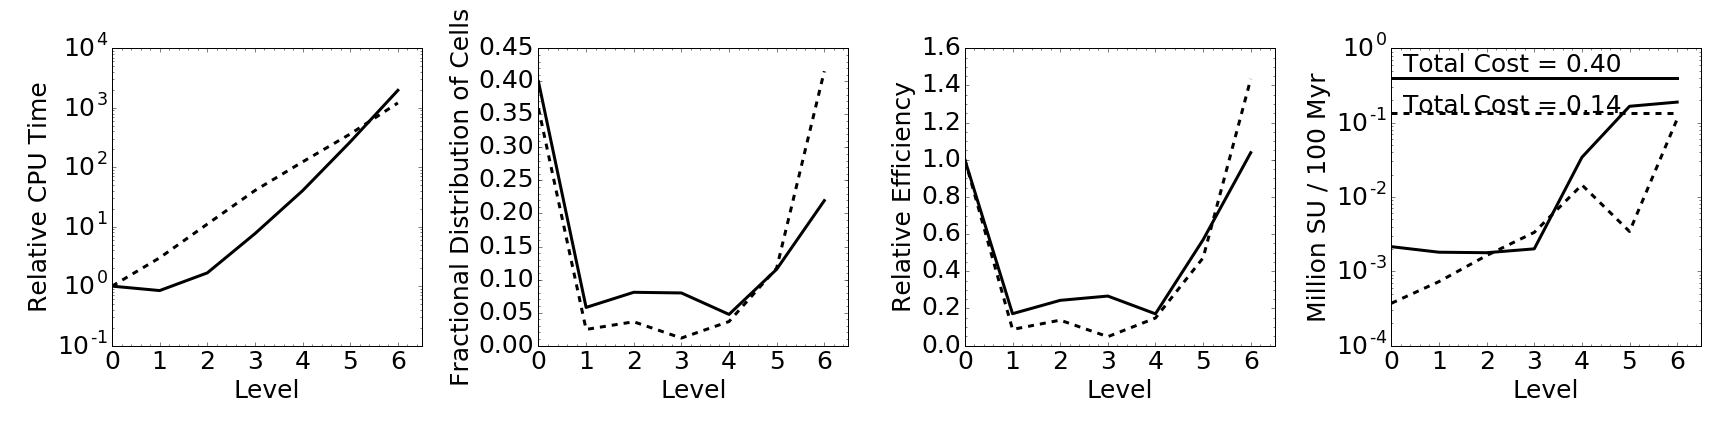
\includegraphics[width=.9\linewidth]{enzo_levels}
\caption{\small Demonstration of grid hierarchy and performance per level on a 1.0 pc (solid) and 2.0 pc (dashed) resolution test of our dwarf galaxy model, each run on 128 processors. For each level, the first panel gives wall time spent, the second the fractional number of cells, the third the efficiency (normalized to the root grid), and the fourth the theoretical lower limit on cost.}
\label{fig:levels}
\end{figure}

Figure~\ref{fig:levels} demonstrates the level-by-level break down of a single cycle in two test simulations with maximum refinement levels of 7 (solid) and 6 (dashed), or 1.0 pc and 2.0 pc resolution respectively. The top panels show that wall time is dominated by computation on the highest level of refinement, in large part because it dominates the cell count across levels, but also because the time step decreases linearly with resolution (not shown). Efficiency varies per level (lower left), but is high for large grid counts, demonstrating effective load-balancing. \texttt{Enzo} reaches typical efficiencies of $\sim 2 \times 10^{4}$ cell updates/s/processor in these test runs. Given these efficiencies and typical values for the time step size on each level (not shown, but is approximately 300 years for level 7 and 600 years for level 6), the bottom right panel shows the estimated SU cost per Gyr of simulation time on 128 processors on the TACC Stampede cluster, assuming all levels operate completely independently (this is a theoretical lower limit on cost). In practice, and as shown in the main document, real cost estimates are a factor of 2-3 higher than this.

%The lower left panel of Figure\ref{fig:levels} provides the relative efficiency of each level, as normalized to the efficiency of level 0. We define efficiency as the number of cell updates per second per processor, with typical values of 10$^4$ as averaged over all levels. The efficiency is determined primarily by the ability of \texttt{Enzo} to properly load balance across all processors, which becomes inefficient if there are too few cells on a given level. For example, levels 1 and 2 have low cell counts and low efficiencies; however, low efficiencies for this reason are generally irrelevant, as very little time is actually spent updating these cells. The efficiency at he highest levels of refinement is generally around $2\times 10^4$ cells/s/proc. Assuming all levels can operate completely independently (which is physically impossible), we present the theoretical lower limit cost of 1 Gyr of simulation time per level on 128 cores in the lower right panel; the horizontal line gives the sum over all levels. To compute this, we adopt typical time steps for each level as obtained from our test simulations using only supernovae feedback and stellar winds. This means a typical time step of roughly 300 years at level 7, and 600 years at level 6. In practice, the levels cannot operate independently; a more realistic estimate is a factor of 2-3 larger than this theoretical minimum.

%\begin{figure}
%\centering
%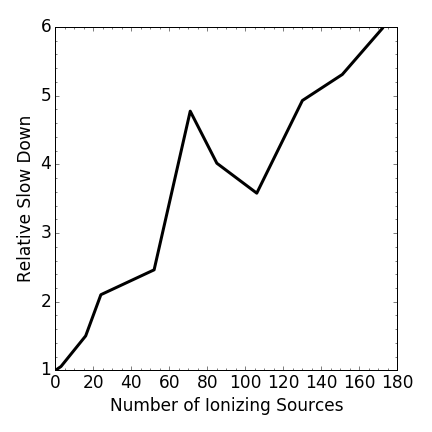
\includegraphics[width=0.45\linewidth]{enzo_radiation}
%\caption{Estimate of relative slow down of a test simulation as a function of the number of ionizing sources. The test simulation is of our dwarf galaxy at 8.0 pc resolution, or a maximum refinement level of 4, run on 32 processors on the TACC Stampede cluster. This test simulation included supernovae, stellar winds, photoelectric heating, and radiative transfer. We estimate that there will be at most a few hundred sources at any one moment in our simulation, implying a maximal slow down of about a factor of 10.}
%\label{fig:radiation}
%\end{figure}

%We demonstrate the effects of including radiative transfer as a function of the number of ionizing particles in Figure~\ref{fig:radiation} for a test simulation run with a maximum refinement level of 4 (8.0 pc resolution) on 64 processors. Shown is the slow down of a given cycle as a function of the number of ionizing sources. We compute this as the number of cell updates per second per particle, normalized to the zero particle case. This implicitly assumes that any decrease in performance is due solely to the number of sources, and no other factors. To be clear, the additional computational time incurred by including radiation is split in into three parts, 1) evolving the photon packages through the grid cells, 2) ray tracing from each source to deposit the photon packages, and 3) communication time communicating photon packages between processors. For this reason, the additional cost also depends upon the nature of the sources themselves, their clustering, and the details of the medium the photons propagate through.

\subsection{Scaling Tests}

\begin{figure}
\centering
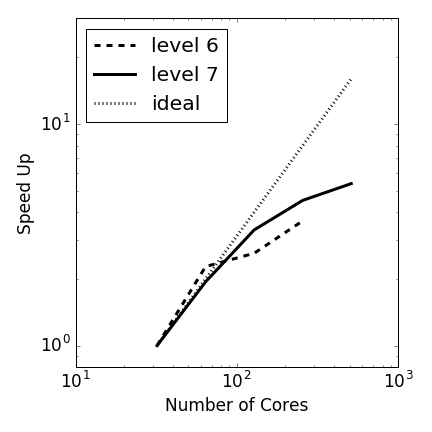
\includegraphics[width=0.4\linewidth]{enzo_scaling}
\caption{\small A demonstration of weak scaling for our two test runs with maximum refinement levels of 6 (dashed) and 7 (solid). Scaling works very well for up to 128 cores, but becomes less than ideal about this amount. We anticipate to run with either 128 or 256 cores for all of our simulations depending on how the grid and particle count evolve in the simulation.}
\label{fig:scaling}
\end{figure}

We demonstrate weak scaling in Figure~\ref{fig:scaling} for our two test simulations, each run with a maximum of 6 and 7 levels of refinement, as compared to ideal scaling. Our simulations scale well up to about 128 processors, falling away from ideal at higher processor counts. However, this is in part because scaling in \texttt{Enzo} works best when the number of root grids on a side is greater than or equal to the number of cores. In this case, we don't expect perfect scaling much above 128 cores for our 128$^3$ simulations. For this reason, we anticipate to run all of our dwarf galaxy models on 128 or 256 cores depending on how the number of cells and particles varies throughout the simulation. We note that \texttt{Enzo} has been shown to scale well to at least 10$^3$ processors in a variety of contexts.

\bibliographystyle{apj}
\bibliography{msbib}


\end{document}
